\documentclass[20pt, a0paper, portrait]{tikzposter}

\usepackage[utf8]{inputenc}
\usepackage[T1]{fontenc}
\renewcommand*\familydefault{\sfdefault}
\usepackage{textcomp}
\usepackage{arev}
\usepackage{arevmath}
\usepackage{arevtext}
\usepackage{graphicx}
\usepackage{wrapfig}
\usepackage{standalone}
\usepackage{microtype}

% Bibliography
\usepackage[backend=biber,
bibencoding=utf8,
bibstyle=numeric-comp,
%style=verbose, %verbose-ibid,
url=true, % include url in reference
doi=true, % include doi in reference
sorting=none, % sorting of citations
%autocite=superscript, % autocite becomes superscript
maxcitenames=1, % Max names displayed when citing in text
maxbibnames=10, % Max number of names displayed in the bibliography
giveninits=true % Use initials
]{biblatex}
\addbibresource{citations.bib}
\renewcommand*{\bibfont}{\footnotesize}

\title{Design Process Models}
\author{Engineering Design \& Manufacture Group}
\date{\today}
\institute{University of Bath, UK}

\usetheme{Default}
\usecolorstyle[colorPalette=GreenGrayViolet]{Default}
\useblockstyle{Default}
\usetitlestyle{Filled}

\begin{document}

\maketitle


\begin{columns}
  \column{0.5}
  \block[]{Introduction}{

    \begin{tikzfigure}[\textcite{wynn2017} mapping of design process models against their scope and type]
      \centering
      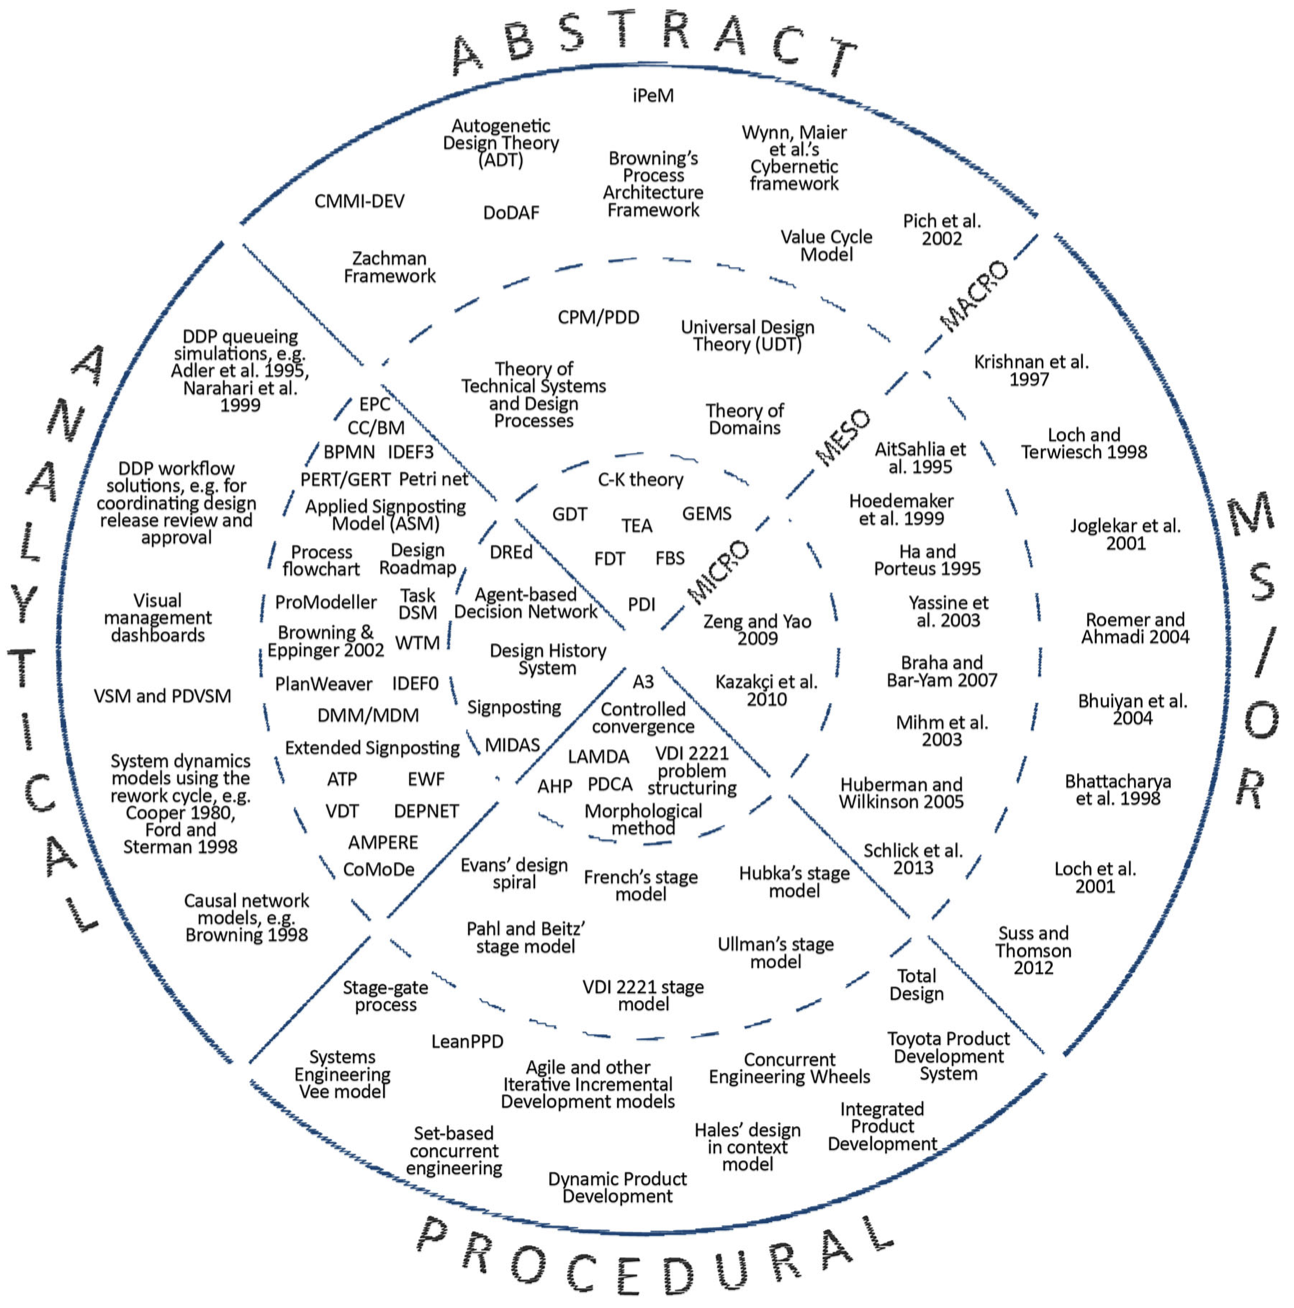
\includegraphics[width=0.16\textwidth]{figures/wynn-review.png}
    \end{tikzfigure}

    Design process models exist at the core of any engineering design exercise. They aid us in defining the approach and the key stages we will take to develop a solution to a given problem. Now, there are a large number of approaches that researchers and industry have developed over the years. \textcite{wynn2017} recent review of process models in design and development revealed that there are over 50 different models, which range from mapping the entire product development process to supporting specific elements of the process. These models also take different perspectives to how Engineering Design should be managed such as abstract, analytical, management science and procedural. 

  }

  \block[]{Stage/Phase-Gate Model}{

    \begin{tikzfigure}[Stage-Gate Model]
      \centering
      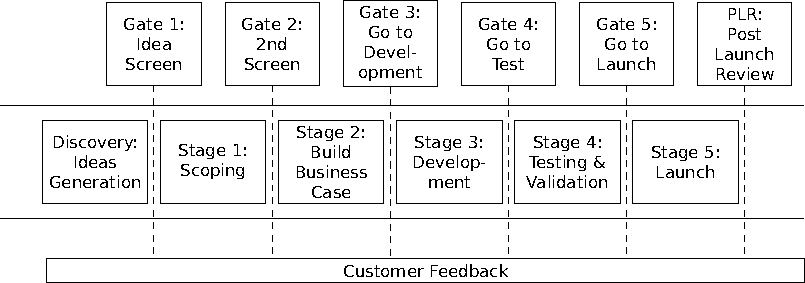
\includegraphics[width=0.4\textwidth]{figures/build/stage-gate.pdf}
      \label{fig-stage}
    \end{tikzfigure}

    Stage/Phase-Gate models arose during the management of large-scale projects for mechanical and chemical engineering in the 1940s. One of the major organisations to develop this model further was in the NASA. NASA introduced its phased review process in the 1960s and broke up the development of their projects into a series of phases that could be individually reviewed.

    \vspace{1em}

    The phased review process consisted of five stage with periodic development reviews between stages (Figure~\ref{fig-stage}). The stages phases are:

  \begin{description}
    \itemsep0em
    \item[Start] Discovery \& Idea Generation
    \item[Stage 1] Scoping
    \item[Stage 2] Building the Business Case
    \item[Stage 3] Development
    \item[Stage 4] Testing \& Validation
    \item[Stage 5] Launch
  \end{description}

  }

  \block[]{V-Model}{

    \begin{tikzfigure}[V-Model]
      \centering
      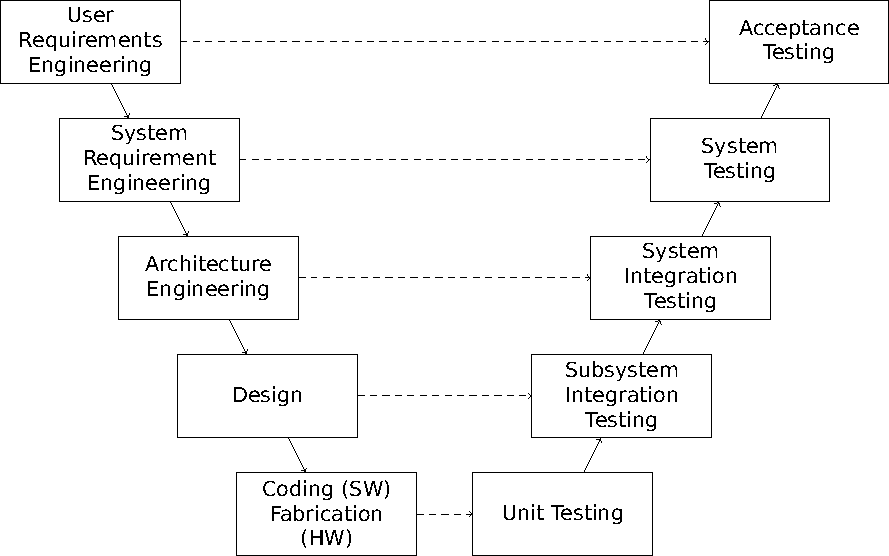
\includegraphics[width=0.3\textwidth]{figures/build/v-model.pdf}
      \label{fig-v-model}
    \end{tikzfigure}

    The V-Model (Figure~\ref{fig-v-model}) has been widely adopted across systems design where a product can be split into separate sub-systems that can be developed and tested independently from one another. The left-hand side of the ``V'' details the processes that organisations follow to decompose the list of requirements for a product into a set of separate system element specifications that are then used to generate a set of designs for the sub-systems of the product.

    \vspace{1em}

    The sub-systems can then be tested independently before being integrated until the full product is formed (right-hand side of the `V'). Testing is performed at each stage of the integration of the systems, which simplifies the identification of issues as the product is built-up.

  }


  \column{0.5}

  \block[]{Systematic Design Process - VDI2221}{

    \begin{tikzfigure}[Systematic Design Approach~\autocite{pahl2013}]
      \centering
      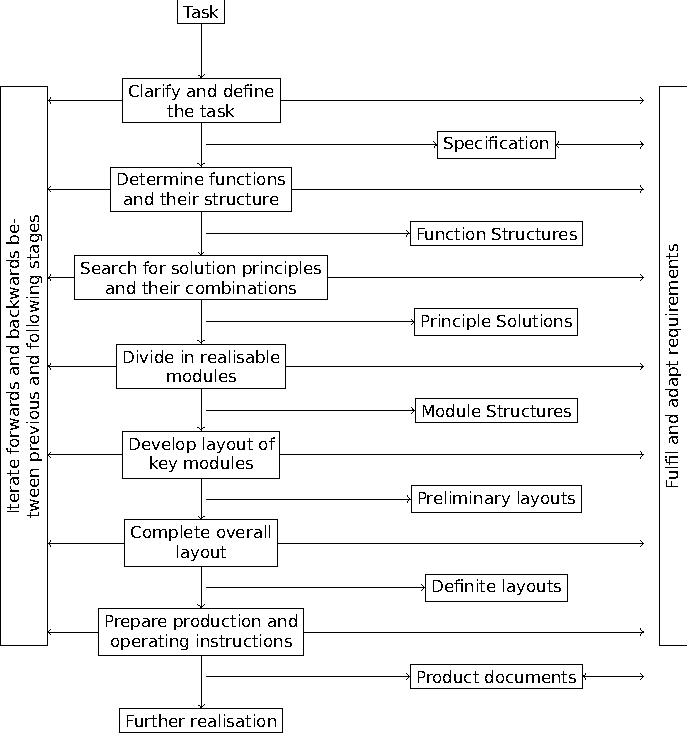
\includegraphics[width=0.28\textwidth]{figures/build/VDI2221.pdf}
      %\includestandalone{figures/VDI2221}
      \label{fig-vdi}
    \end{tikzfigure}

    VDI2221 was developed by senior designers from industry and academia. The aim was to provide a generic approach for the design of products within the fields of mechanical, precision, control, software and process engineering. The approach (Figure~\ref{fig-vdi}) includes seven basic working steps.

    \vspace{1em}

    As this process was designed for general applicability, the VDI2221 has a very abstract structure, thus permitting product-specific and company-specific variations. Figure~\ref{fig-vdi} should therefore be regarded as a guideline to which detailed working procedures can be assigned. Special emphasis is placed on the iterative nature of the approach and the sequence of the steps must not be considered rigid. Some steps might be omitted, and others repeated frequently. This flexibility is in accordance with practical design experience and enables companies to frame their processes in a similar manner to enable communication of where they are in their product development cycle. 

  }

  \block[]{Design Double Diamond}{

    \begin{tikzfigure}[Design Double Diamond]
      \centering
      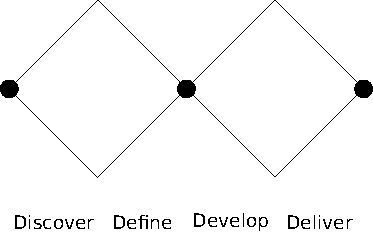
\includegraphics[width=0.15\textwidth]{figures/build/double-diamond.pdf}
      \label{fig-dd}
    \end{tikzfigure}

    The Design Council~\autocite{council2007} illustrates the design process as a Double Diamond (Figure~\ref{fig-dd}), which is divided into four distinct phases: Discover; Define; Develop and, Deliver.

    \vspace{1em}
    
    In all creative processes a number of possible ideas are created (`divergent thinking') before refining and narrowing down to the best idea (`convergent thinking'), and this can be represented by a diamond shape. The Double Diamond indicates that this happens twice – once to confirm the problem definition and once to create the solution. One of the greatest mistakes is to omit the left-hand diamond and end up solving the wrong problem.

    \vspace{1em}
    
    In order to discover which ideas are best, the creative process is iterative. This means that ideas are developed, tested and refined a number of times, with weak ideas dropped in the process. This cycle is an essential part of good design.

    \vspace{1em}
    
    Practical design methods -- like user diaries, journey mapping and character profiles -- move a project through the four phases of the Double Diamond. 

    \vspace{1em}
    
    \textbf{Discover} The first quarter of the Double Diamond model covers the start of the project. Designers try to look at the world in a fresh way, notice new things and gather insights.
    
    \textbf{Define} The second quarter represents the definition stage, in which designers try to make sense of all the possibilities identified in the Discover phase. Which matters most? Which should we act on first? What is feasible? The goal here is to develop a clear creative brief that frames the fundamental design challenge.
    
    \textbf{Develop} The third quarter marks a period of development where solutions or concepts are created, prototyped, tested and iterated. This process of trial and error helps designers to improve and refine their ideas.
    
    \textbf{Delivery} The final quarter of the double diamond model is the delivery stage, where the resulting project (a product, service or environment, for example) is finalised, produced and launched.

  }


  \block[]{References}{
    \printbibliography[heading=none]{}
  }
\end{columns}





\end{document}